\documentclass[10pt,twocolumn]{witseiepaper}

% All KJN's macros and goodies (some shameless borrowing from SPL)

\usepackage{KJN}


\usepackage{verbatim} % for writing code in the text
\usepackage{tikz} % for drawing stuff
\usetikzlibrary{positioning} % for relative coordinates

\usepackage{listings} %for including code
\usepackage{golang}  % include custom language for Go.
\usepackage{gostyle} % include custom style for Go.
\usepackage{graphicx}
\usepackage{subfig}

\pagestyle{plain}

\addtolength{\oddsidemargin}{-.2in}
\addtolength{\evensidemargin}{-.2in}
\addtolength{\textwidth}{0.4in}

% PDF Info
\ifpdf
\pdfinfo{
/Title  (ELEN4017 Project Report)
/Author (James Allingham and Devin Taylor)
}
\fi

%%%%%%%%%%%%%%%%%%%%%%%%%%%%%%%%%%%%%%%%%%%%%%%%%%%
\begin{document}


\title{Implementation of the HTTP Protocol in Go \\ ELEN4017 Project Report}

\author{James Allingham (672732) and Devin Taylor (603956)}
\thanks{School of Electrical \& Information Engineering, University of the
Witwatersrand, Private Bag 3, 2050, Johannesburg, South Africa}



%%%%%%%%%%%%%%%%%%%%%%%%%%%%%%%%%%%%%%%%%%%%%%%%%%%
\abstract{}

\keywords{}


\maketitle
%\thispagestyle{empty}

%%%%%%%%%%%%%%%%%%%%%%%%%%%%%%%%%%%%%%%%%%%%%%%%%%%%
\section{INTRODUCTION}

%%%%%%%%%%%%%%%%%%%%%%%%%%%%%%%%%%%%%%%%%%%%%%%%%%%%
\section{BACKGROUND}

%%%%%%%%%%%%%%%%%%%%%%%%%%%%%%%%%%%%%%%%%%%%%%%%%%%%
\section{HTTP DESCRIPTION}

The Hyper Text Transfer Protocol has been in existence since 1990 \cite{rfc7230}. It is used by the World Wide Web as an application level protocol for transfer of information in a distributed system. It consists of two programs: a client and a server. The client, also commonly referred to as the browser, communicates with the server by sending it a HTTP request message. The server then responds with a HTTP response message. HTTP is a stateless protocol which means that the server has no knowledge of the client other than the information contained in the request. This is a limitation of HTTP which is overcome with the use of cookies \cite{kurose}. HTTP uses Transmission Control Protocol (TCP) as its underlying transport layer protocol \cite{kurose}. This means that HTTP does not need to worry about reliable data transfer issues such as out of sequence packets or packet loss.  

A typical HTTP communication can be described as follows: 
\begin{enumerate}
	\item A server sets up a TCP listener on one of its ports (an end point for network communication). The default port to HTTP is 80. 
	\item A client initiates a TCP connection with the server (via the server's url) on the appropriate port. 
	\item The client and server complete a `three way handshake' after which each of them have a socket (a virtual data connection between processes) which can be used to send and receive messages. Note that the port associated with these sockets will not be 80.
	\item The client sends a HTTP request message to the server using its socket. This request is received by the server on its matching socket.
	\item The server processes the request and sends an appropriate HTTP response to the client. This communication once again makes use of the sockets that have been set up. 
	\item The server closes the TCP connection.
	\item The client receives the HTTP response before the connection is closed.
\end{enumerate}

	\subsection{Request and Response Messages} \label{formats}

	HTTP is based on communication via request and response messages, both of which have specific formats and can take on a number of values. Both request and response messages contain three parts: the request/ response line, zero or more header lines and an optional body. The format of an HTTP request is shown in \figref{reqformat}. A number of common HTTP request methods are described in \tabref{httpreqs}. The format of an HTTP response is shown in \figref{respformat}. A number of common HTTP response codes are described in \tabref{httpresps}. 2xx responses indicate a success, 3xx responses indicate that client must submit a new request, 4xx responses indicate that the client is in error and 5xx responses indicate that the server is in error.

	\begin{figure}[htbp]
	\centering
		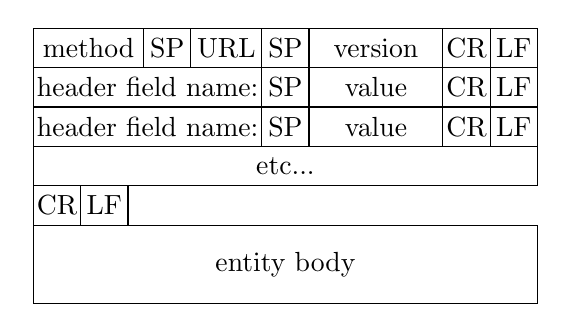
\begin{tikzpicture}
			\draw 
				(0,0) rectangle (1.4,-0.5) node[pos=.5] {method}
				(1.4,0) rectangle (2.0,-0.5) node[pos=.5] {SP}
				(2.0,0) rectangle (2.9,-0.5) node[pos=.5] {URL}
				(2.9,0) rectangle (3.5,-0.5) node[pos=.5] {SP}
				(3.5,0) rectangle (5.2,-0.5) node[pos=.5] {version}
				(5.2,0) rectangle (5.8,-0.5) node[pos=.5] {CR}
				(5.8,0) rectangle (6.4,-0.5) node[pos=.5] {LF}
				(0,-0.5) rectangle (2.9,-1) node[pos=.5] {header field name:}
				(2.9,-0.5) rectangle (3.5,-1) node[pos=.5] {SP}
				(3.5,-0.5) rectangle (5.2,-1) node[pos=.5] {value}
				(5.2,-0.5) rectangle (5.8,-1) node[pos=.5] {CR}
				(5.8,-0.5) rectangle (6.4,-1) node[pos=.5] {LF}
				(0,-1) rectangle (2.9,-1.5) node[pos=.5] {header field name:}
				(2.9,-1) rectangle (3.5,-1.5) node[pos=.5] {SP}
				(3.5,-1) rectangle (5.2,-1.5) node[pos=.5] {value}
				(5.2,-1) rectangle (5.8,-1.5) node[pos=.5] {CR}
				(5.8,-1) rectangle (6.4,-1.5) node[pos=.5] {LF}
				(0,-1.5) rectangle (6.4, -2) node[pos=.5] {etc...}
				(0,-2) rectangle (0.6,-2.5) node[pos=.5] {CR}
				(0.6,-2) rectangle (1.2,-2.5) node[pos=.5] {LF}
				(0,-2.5) rectangle (6.4,-3.5) node[pos=.5] {entity body}
				;
		\end{tikzpicture}
		\caption{HTTP request format}
		\label{reqformat}
	\end{figure}

	\begin{table*}[tb]
		\centering
		\caption{Commonly used HTTP request methods}
		\label{httpreqs}
		\begin{tabular}{p{0.1\textwidth}|p{0.8\textwidth}}
			\hline
			\textbf{Method} & \textbf{Description} \\ \hline
			GET & Request data from the specified URL \\
			HEAD & Request a response identical to the GET response but without the body so that the client can get the header values without retrieving the entire data \\
			POST & Request that the web server accept the data in body, this is often used for filling in forms\\
			PUT & Request that the web server store the data in the body at the specified URL \\
			DELETE & Request that the web server remove the resource stored at the specified URL  \\
			TRACE & Request that the web server echo the request so that the client can detect any changes made to the original request \\
			OPTIONS & Request that the web server inform the client which methods are valid at the specified URL \\
			PATCH & Request that the web server apply a partial change to the resource at the given URL \\
			\hline
		\end{tabular}
	\end{table*}

	\begin{figure}[htbp]
	\centering
		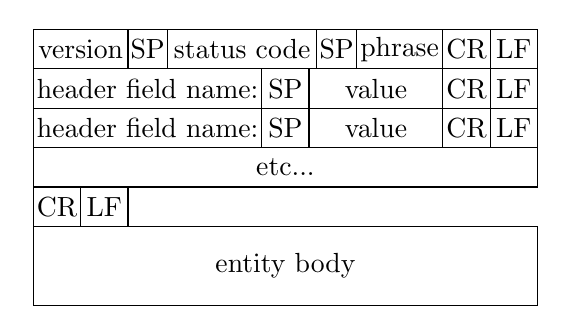
\begin{tikzpicture}
			\draw 
				(0,0) rectangle (1.2,-0.5) node[pos=.5] {version}
				(1.2,0) rectangle (1.7,-0.5) node[pos=.5] {SP}
				(1.7,0) rectangle (3.6,-0.5) node[pos=.5] {status code}
				(3.6,0) rectangle (4.1,-0.5) node[pos=.5] {SP}
				(4.1,0) rectangle (5.2,-0.5) node[pos=.5] {phrase}
				(5.2,0) rectangle (5.8,-0.5) node[pos=.5] {CR}
				(5.8,0) rectangle (6.4,-0.5) node[pos=.5] {LF}
				(0,-0.5) rectangle (2.9,-1) node[pos=.5] {header field name:}
				(2.9,-0.5) rectangle (3.5,-1) node[pos=.5] {SP}
				(3.5,-0.5) rectangle (5.2,-1) node[pos=.5] {value}
				(5.2,-0.5) rectangle (5.8,-1) node[pos=.5] {CR}
				(5.8,-0.5) rectangle (6.4,-1) node[pos=.5] {LF}
				(0,-1) rectangle (2.9,-1.5) node[pos=.5] {header field name:}
				(2.9,-1) rectangle (3.5,-1.5) node[pos=.5] {SP}
				(3.5,-1) rectangle (5.2,-1.5) node[pos=.5] {value}
				(5.2,-1) rectangle (5.8,-1.5) node[pos=.5] {CR}
				(5.8,-1) rectangle (6.4,-1.5) node[pos=.5] {LF}
				(0,-1.5) rectangle (6.4, -2) node[pos=.5] {etc...}
				(0,-2) rectangle (0.6,-2.5) node[pos=.5] {CR}
				(0.6,-2) rectangle (1.2,-2.5) node[pos=.5] {LF}
				(0,-2.5) rectangle (6.4,-3.5) node[pos=.5] {entity body}
				;
		\end{tikzpicture}
		\caption{HTTP request format}
		\label{respformat}
	\end{figure}

	\begin{table*}[tb]
		\centering
		\caption{Commonly used HTTP response methods}
		\label{httpresps}
		\begin{tabular}{p{0.05\textwidth}|p{0.275\textwidth}|p{0.55\textwidth}}
			\hline
			\textbf{Code} & \textbf{Phrase} & \textbf{Meaning} \\ \hline
			200 & OK & HTTP request successful \\
			201 & Created & A new resource was created \\
			202 & Accepted & Request has been accepted for processing \\
			301 & Moved Permanently & The requested resource is now located elsewhere \\
			302 & Found & The requested resource is temporarily located elsewhere \\
			304 & Not Modified & The requested resource has not been modified since last requested - used for caching \\
			400 & Bad Request & The request was not understood by the server \\
			404 & Not Found & The requested resource could not be found \\
			505 & HTTP Version Not Supported & The server does not support the HTTP version of the request \\
			\hline
		\end{tabular}
	\end{table*}

	\subsection{Persistent and Non-persistent} \label{pvnp}

	In HTTP version 1.0 (HTTP/1.0), all communication takes the form shown above \cite{rfc1945}. In other words a new TCP connection is made every time the client wants to make a request to the server. However, this approach has its disadvantages. The primary disadvantage is that it is wasteful to repeatedly make new connections when more than one request is going to be made. This is because setting up the TCP connection requires the three way handshake which is a time consuming operation. The solution to this, which was implemented in HTTP version 1.1 (HTTP/1.1), was to allow connections to persist for multiple request-response pairs \cite{rfc7230}. This is accomplished using the \emph{connection} header field, which can take on the values \emph{close} and \emph{keep-alive} for non-persistent and persistent connections respectively.

	\subsection{Proxy Servers and Caching}

	Another limitation of HTTP that results from its statelessness is that it does not have a mechanism for `smart' communication. Consider the following situation:

	\begin{enumerate}
		\item A client requests the file \verb|Foo.bar|.
		\item The server responds by sending the file to the client by encapsulating it withing an HTTP response message.
		\item The same client receives the file and immediately requests the same file, \verb|Foo.bar|, again.
		\item The server responds by sending the exact same file to the client again.
	\end{enumerate} 

	The problem with the above situation is that the server is wasting time sending the client the file \verb|Foo.bar| again because no changes have been made to the file. As a result the server could be slower to respond to other clients. This also increases congestion on the uplink of the Local Area Network of the client. The solution is to make use of a Proxy server (proxy), also known as a web cache. In this situation all HTTP requests are sent to the proxy by default. The proxy then forwards requests to the destination servers. The proxy acting as an intermediary between the clients and server can now store files sent from a server to a client. Now when a client requests the same file in quick succession, the server need only send it once. This solves both problems: the server has a reduced load and the uplink traffic is also reduced. Additionally, because LANs usually have network speeds orders of magnitude larger than the uplink, the client gets the data faster. By making use of the \emph{Last-Modified} and \emph{If-Modified-Since} headers, the proxy can make sure that it always serves the client with the most up to date version of the requested file. This is accomplished with the \emph{Conditional-Get} request. 	

	\subsection{User Datagram Protocol}

	Although HTTP makes use of TCP as it's transport layer protocol, a HTTP-like communication system can be implemented with the User Datagram Protocol (UDP). This would have the disadvantage that it provides unreliable communication. However, it could be faster than if TCP were used.


%%%%%%%%%%%%%%%%%%%%%%%%%%%%%%%%%%%%%%%%%%%%%%%%%%%%
\section{SYSTEM OVERVIEW}

	\subsection{System Architecture}

	As mentioned, the HTTP protocol follows the Client-Server model. This means that to properly demonstrate the implementation of HTTP, both a client and server are required. Additionally, in order to more extensively represent a real world application of HTTP, a proxy is required. All three of these systems have been implemented in the Go programming language developed by Google. It is a statically typed, imperative, garbage collected, compiled language. It was designed as a system programming language with specific support for networking and multi-threading.

	\subsubsection{Client:}

	The client is responsible for sending HTTP requests to the server. These requests are generated based on user input. This process involves creating the HTTP request in the correct format, as discussed in \secref{formats}, creating a TCP or UDP connection and then sending the request in byte format. The client then waits for a response from the server, decomposing the response into its elements various elements, mentioned in \secref{formats}, and taking an appropriate action based on the response type and contents.

	\subsubsection{Server:}

	The server is responsible for listening for both TCP and UDP connections. Once a connection of either kind is made, the server must handle the client which involves, in the case of TCP, creating a new socket for the communication, and in the case of either TCP or UDP, receiving the HTTP request. The HTTP request must then be decomposed into its elements, discussed in \secref{formats}. Based on the type of request and its contents, the server must take an appropriate action as well as compose and send a HTTP response. Then, in the case of non-persistent TCP connections only, the sever must close the connection.

	\subsubsection{Proxy Server:}

	The proxy is responsible for taking all incoming requests from the client and forwarding them to the destination server. The proxy server must also cache web objects sent, via its self, from the server to the client. This makes use of the \verb|If-Modified-Since| and \verb|Last-Modified| header fields to allow the proxy to have the most up to date version of any object in its cache. The proxy acts as both a client and a server in the sense that it is viewed as a server from the perspective of the client and vice versa. As a result it has many of the responsibility listed above.

\subsection{Features}

A number of features were implemented. The ability to use both TCP and UDP was implemented for the client and server. The ability to use both persistent and non-persistent TCP was implemented on the client, server and proxy. Multi-threading was implemented on the server and proxy allowing them to server multiple clients. The ability to track the round-trip-time (RTT) of a message was implemented on the client.

	\subsubsection{TCP vs UDP:}

	This feature allows the user of the client to select the underlying transport layer protocol to use. TCP has the advantage that it offers some robustness in the form of protection against packet loss and delay. On the other hand UDP offers a higher speed than TCP due to its lack of data reliability services. The server implements this feature in terms of the ability to listen for both TCP and UDP connections and handle each appropriately. 

	\subsubsection{Persistent vs Non-persistent:}

	The choice of persistent TCP over non-persistent TCP allows the communication between the client and the server to be sped up for sessions with more than one request. This speed up is a result of not having to perform the three-way handshake every time a request message is sent from the client to the server. This is implemented using the header fields discussed in \secref{pvnp} as well as Multi-threading discussed below in \secref{thread}.

	\subsubsection{Multi-threading:} \label{thread}

	Multi-threading, implemented via \verb|goroutines|, allows the server (as well as the proxy) to be parallelized. Effectively, this feature allows the server to handle multiple TCP connections at the same time (while also serving clients via UDP connections). This makes the use of persistent TCP feasible as it allows the server to keep listening for new TCP connections even while handling a long persistent communication with the client.

	\subsubsection{RTT timer:}

	This feature allows the client to time how long it takes to recieve the response to a message. This could be useful for time out periods or for comparing different types and combinations of communication schemes i.e. TCP vs UDP, persistent vs non-persistent, and proxy vs no proxy.

%%%%%%%%%%%%%%%%%%%%%%%%%%%%%%%%%%%%%%%%%%%%%%%%%%%%
\section{DETAILED IMPLEMENTATION}

%%%%%%%%%%%%%%%%%%%%%%%%%%%%%%%%%%%%%%%%%%%%%%%%%%%%
\section{DIVISION OF WORK}

%%%%%%%%%%%%%%%%%%%%%%%%%%%%%%%%%%%%%%%%%%%%%%%%%%%%
\section{RESULTS}

	In order to test the integrity of the system it was necessary to observer the behaviour of the system between two computers over the same network. The primary criteria for testing the system was to ensure the following:

	\begin{itemize}
		\item The client request message was received by the server and interpreted correctly.
		\item The server response message was received by the client in conjunction with the necessary data and interpreted correctly.
		\item The client was able to respond to the contents of the servers message by either following a link to the actual site or requesting further information in the form of sources.
		\item The server was capable of returning conditional error codes if necessary.
		\item The client was able to interact with the proxy.
		\item The proxy was able to interact with the client.
		\item The proxy was able to interact with the cache and communicate the corresponding information with the client and server respectively.
	\end{itemize}

	\subsection{Basic Client Server HTTP Requests and Responses} % (fold)
	\label{sub:basic_client_server}
		
		As mentioned in Table~\ref{httpreqs} there are a set of commonly user HTTP requests. For the basis of the project only GET, HEAD, POST, PUT and DELETE were required to be implemented. The use of Wireshark allowed for the message trace between the client and server to be followed. It also provides detailed insight into the communications by being able to analyse the messages being sent and received.
		
		\subsubsection*{The GET Request}: With reference to Figure~\ref{fig:basic_get} of Appendix~\ref{sub:wireshark_results} the client sends a GET request to the server, to which the server responds with an OK message containing the contents of the file that was requested. The OK message symbolises that the server was able to access the requested file. The second get message sent for \texttt{/test.jpg} is due to the fact that the returned file contained an image and as a result the client is able to detect the presence of sources and request them from the applicable server. \\
		
		An example of the GET message sent can be seen in Figure~\ref{fig:basic_get_message} of Appendix~\ref{sub:wireshark_results}. The aspects of interest are the inclusion of the required URI as well as the method (GET). This is contrary to what is observed in Figure~\ref{fig:basic_get_response} whereby there is no mention of a URI but there is the inclusion of the \texttt{Data} section which contains the requested content. These two images highlight the fundamental differences between the HTTP messages sent by the client and the HTTP messages sent by the server.
		
		\subsubsection*{The HEAD Request}: 
	% subsubsection basic_client_server_http_requests_and_responses (end)
%%%%%%%%%%%%%%%%%%%%%%%%%%%%%%%%%%%%%%%%%%%%%%%%%%%%
\section{CRITICAL ANALYSIS}

%%%%%%%%%%%%%%%%%%%%%%%%%%%%%%%%%%%%%%%%%%%%%%%%%%%%
\section{DESCRIPTION OF CODE}

%\lstinputlisting[language=go, style=go, breaklines=true]{../../src/client/client.go}

%%%%%%%%%%%%%%%%%%%%%%%%%%%%%%%%%%%%%%%%%%%%%%%%%%%

\section{CONCLUSION}

%%%%%%%%%%%%%%%%%%%%%%%%%%%%%%%%%%%%%%%%%%%%%%%%%%%

\begin{thebibliography}{1}

\bibitem{rfc7230} Fielding R, Reschke J. `Hypertext Transfer Protocol (HTTP/1.1): Message Syntax and Routing.' IETF, RFC June 2014. [online] Available: \url{https://tools.ietf.org/html/rfc7230}

\bibitem{kurose} Kurose, J F, Ross K W (2013). \emph{Computer networking: a top-down approach.} Boston, Pearson. pp 83 - 115.

\bibitem{rfc1945} Berners-Lee T, Fielding R, Frystyk H. `Hypertext Transfer Protocol -- HTTP/1.0' IETF, RFC May 1996. [online] Available: \url{https://tools.ietf.org/html/rfc1945}

\end{thebibliography}

%%%%%%%%%%%%%%%%%%%%%%%%%%%%%%%%%%%%%%%%%%%%%%%%%%%
\clearpage
\onecolumn
\appendix
\section{Results supporting information} % (fold)
\label{sec:results}
	
	This appendix details the results obtained when running the application one two separate computers on the same network. The results include excerpts of the results obtained from Wireshark as well as the Round Trip Times (RTT) obtained for different implementations of the project.

	\subsection{Wireshark results} % (fold)
	\label{sub:wireshark_results}
	
		\begin{figure}
			\centering
			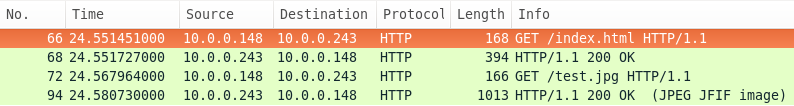
\includegraphics[width=\columnwidth]{resources/get_html}
			\caption{Computer interaction for GET request}
			\label{fig:basic_get}
		\end{figure}
		
		\begin{figure}
			\centering
			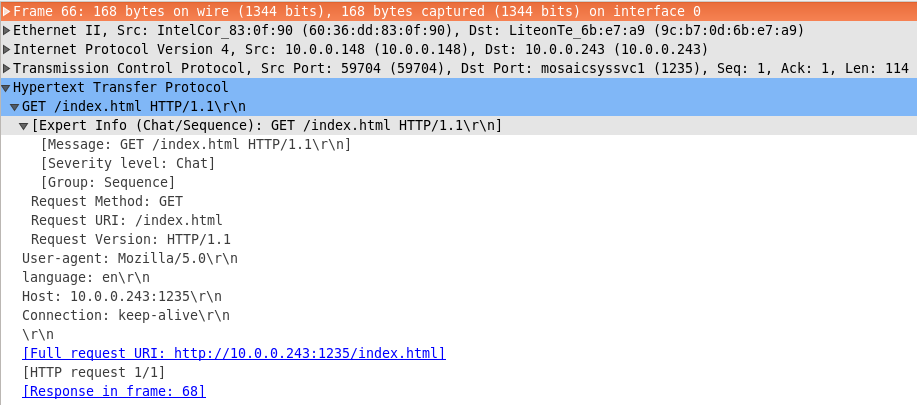
\includegraphics[width=\columnwidth]{resources/message_get_html}
			\caption{GET request message}
			\label{fig:basic_get_message}
		\end{figure}
		
		\begin{figure}
			\centering
			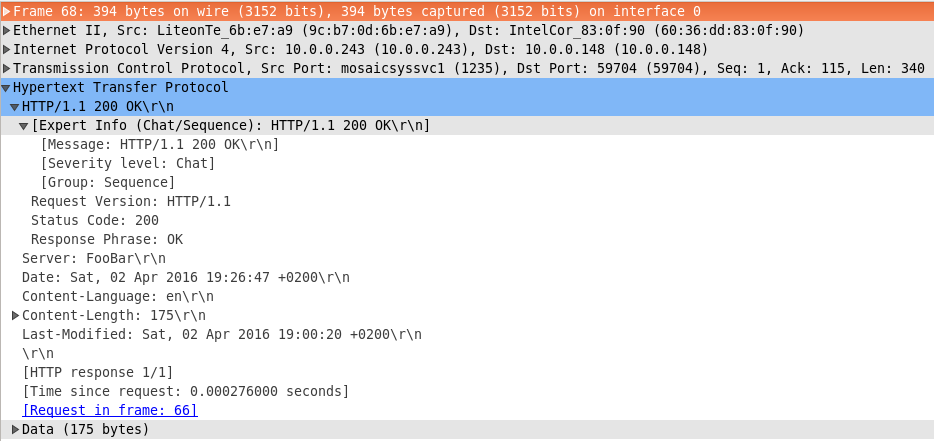
\includegraphics[width=\columnwidth]{resources/message_get_response_html}
			\caption{GET response message}
			\label{fig:basic_get_response}
		\end{figure}
		
%		\begin{figure}
%			\centering
%			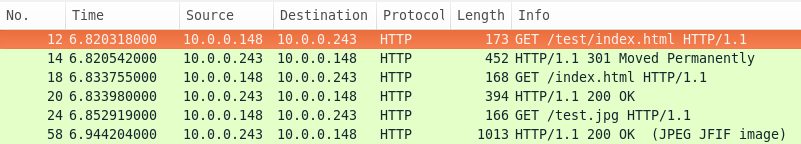
\includegraphics[width=\columnwidth]{resources/301.png}
%			\caption{Computer interaction for 301 status code}
%			\label{fig:301}
%		\end{figure}


	% subsubsection wireshark_results (end)


% section results (end)

\end{document}